% Исследовательская часть
\section{Исследовательская часть}

\hspace{1.25cm}
В данном разделе буду рассмотрены результаты работы программы на разных входных данных, а также проведены сравнения параллельной и последовательной работы программы и ускорения, связанного с распараллеливанием.


\subsection{Примеры работы программы}

\hspace{1.25cm}
На рисунке~\ref{fig:example_0_0_0} представлена работа программы при введённых двух окнах, двери и стене при углах наклона сцены 0 градусов по всем осям.

\begin{figure}[H]
    \centering
    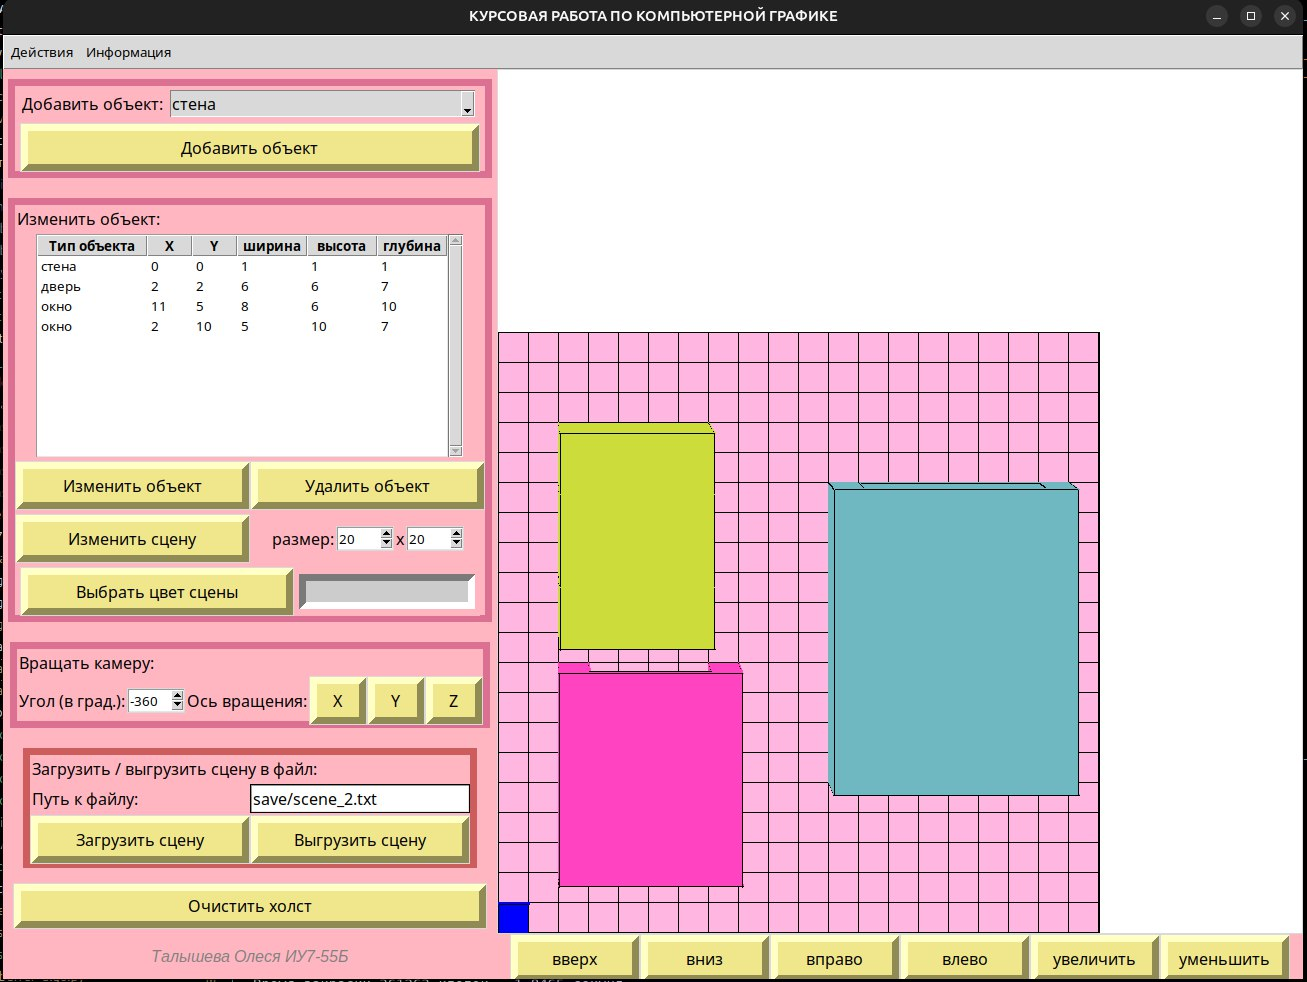
\includegraphics[width=1\textwidth]{img/example_0_0_0.png}
    \caption{Работа программы при введённых двух окнах, двери и стене при углах наклона сцены 0 по всем осям.}
    \label{fig:example_0_0_0}
\end{figure}

На рисунке~\ref{fig:example_60_30_0} представлена работа программы при введённых двух окнах, двери и стене при углах наклона сцены 60, 30 и 0 градусов по осям x, y и z соответственно.

\begin{figure}[H]
    \centering
    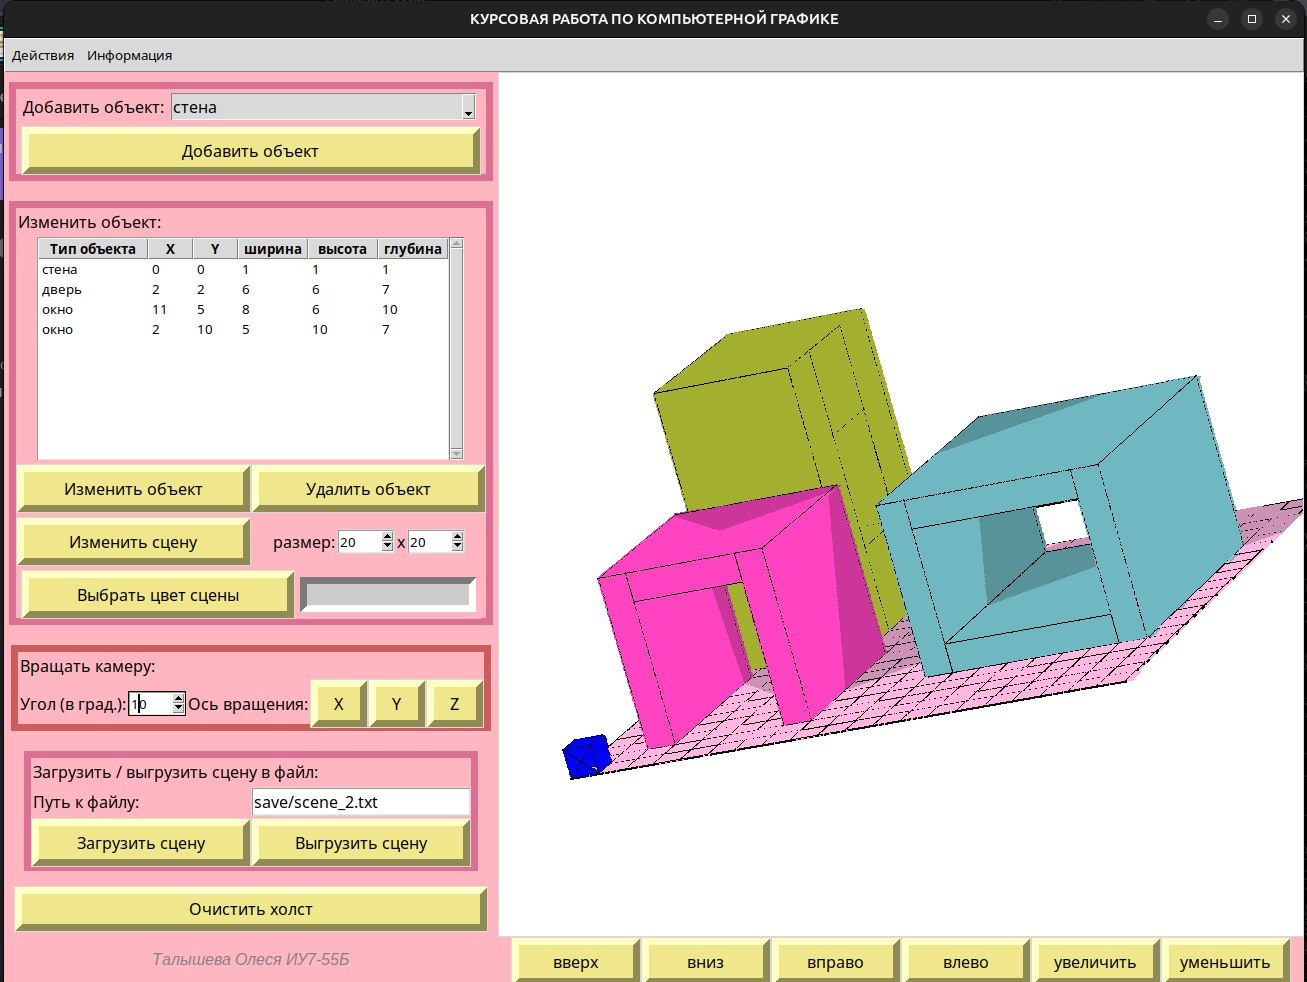
\includegraphics[width=1\textwidth]{img/example_60_30_0.png}
    \caption{Работа программы при введённых двух окнах, двери и стене при углах наклона сцены 60, 30 и 0 градусов по осям x, y и z соответственно.}
    \label{fig:example_60_30_0}
\end{figure}

На рисунке~\ref{fig:example_60_90_0} представлена работа программы при введённых двух окнах, двери и стене при углах наклона сцены 60, 90 и 0 градусов по осям x, y и z соответственно.

\begin{figure}[H]
    \centering
    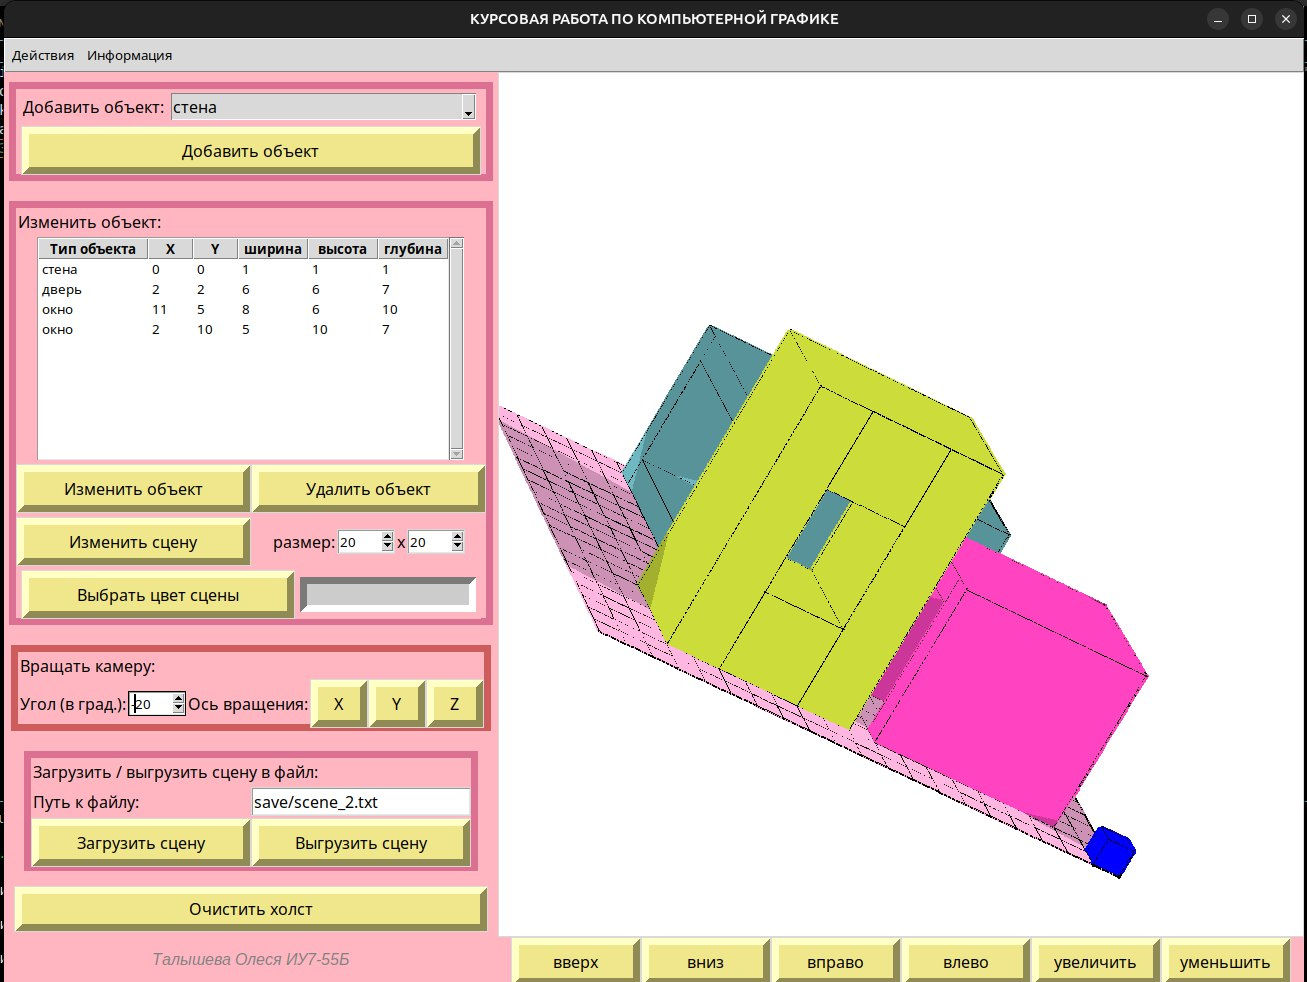
\includegraphics[width=1\textwidth]{img/example_60_90_0.png}
    \caption{Работа программы при введённых двух окнах, двери и стене при углах наклона сцены 60, 90 и 0 градусов по осям x, y и z соответственно.}
    \label{fig:example_60_90_0}
\end{figure}


\subsection{Результат сравнения времени работы программы}

\hspace{1.25cm}
На рисунке~\ref{fig:test_calc_pixel_matrix_performance} представлено сравнение последовательного и параллельного сбора информации для матрицы пикселей Z-буфера для удаления невидимых линий и теневого Z-буфера для времени работы программы.

\begin{figure}[H]
    \centering
    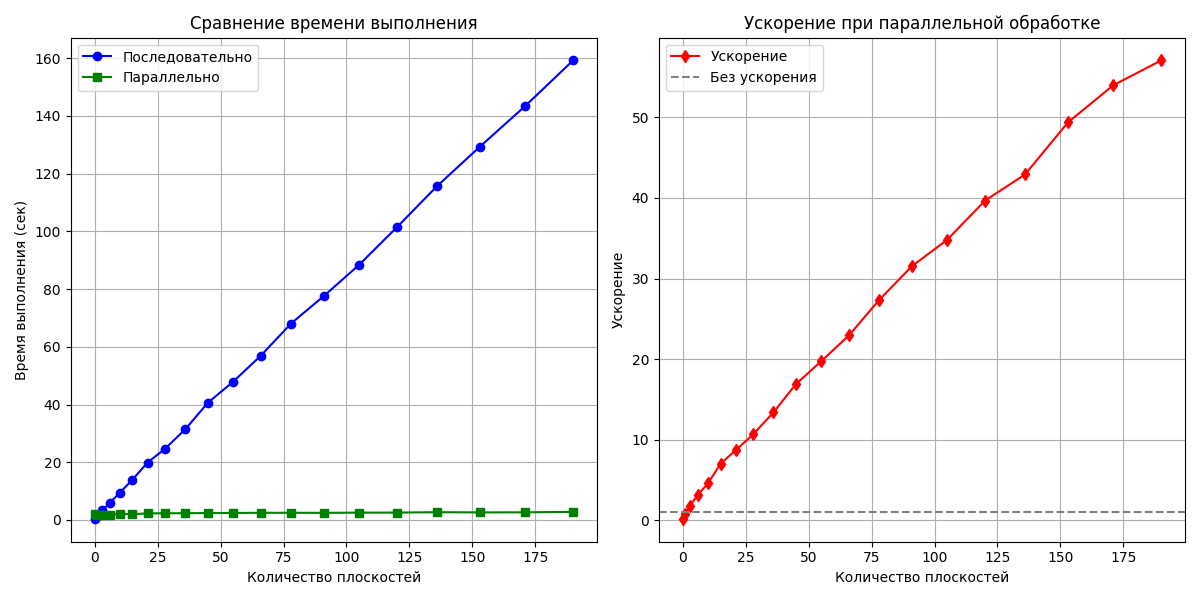
\includegraphics[width=1\textwidth]{img/test_calc_pixel_matrix_performance.png}
    \caption{Графики сравнения времени работы программы.}
    \label{fig:test_calc_pixel_matrix_performance}
\end{figure}

Левый график отображает время выполнения программы при последовательном (синяя кривая) и при параллельном вычислении Z-буфера (зелёная кривая). Для последовательного режима время выполнения линейно возрастает с увеличением числа плоскостей. Для параллельного режима время выполнения остаётся практически постоянным, с незначительными изменениями при увеличении числа плоскостей.

Правый демонстрирует ускорение работы программы при параллельной обработке (красная кривая). Таким образом, ускорение возрастает по мере увеличения числа плоскостей, что отражает эффективность параллельной обработки. При большом количестве плоскостей ускорение достигает значительных значений (более 140 раз).


\subsection{Выводы}

\hspace{1.25cm}
По приведённым исследованиям видно, что:

\begin{enumerate}
\item Параллельная обработка значительно превосходит последовательную по времени выполнения, особенно при увеличении числа плоскостей.

\item Ускорение параллельной программы почти линейно растёт с увеличением числа задач, что подтверждает эффективность параллелизации.

\item Для небольшого числа плоскостей выигрыш от параллелизации менее заметен из-за накладных затрат на управление потоками.

\item Для больших объёмов задач параллельная программа демонстрирует почти идеальное масштабирование.
\end{enumerate}

Следовательно, включение параллельной обработки позволяет существенно сократить время выполнения ресурсоёмких задач.

\newpage